\section{DGFE Theory}

We begin with equation \ref{g_mu_treq}; the within group $g$, within angle $n$ 1D transport equation.  In the following section we drop the group subscript and angle superscript and set $Q(x)=0$.

\begin{equation}
\mu \frac{\partial}{\partial x} \psi(x) + \Sigma_t \psi(x) = S(x)
\label{1d_tr_dg}
\end{equation}
Equation \ref{1d_tr_dg} is a first order, linear, hyperbolic ordinary differential equation, as such the methods introduced in chapter 6
(even parity transport) of E. E. Lewis’s computational methods in radiation transport largely do not apply. The even parity formulation of the transport equation contains a spatial derivative of order 2 results
in certain nice aspects to the DGFE discretized equations – primarily that even order equations yield
symmetric matrices after discretization. The even parity formulation of the transport equation is not pursued here
since it has difficulty including anisotropic scatter \cite{Lewis}. It is possible to use the Petrov-Galerkin method
on the first order equation without constructing the second order form of the transport equation.

First, we multiply both sides of equation \ref{1d_tr_dg} by a yet to be defined test function, $v(x)$ resulting in:
\begin{equation}
\mu \frac{\partial}{\partial x} \psi(x) v(x) + \Sigma_t \psi(x)v(x) = S(x)v(x)
\label{1d_tr_dg2}
\end{equation}
Next the equation is integrated over the domain, $x \in [0, L]$:
\begin{equation}
\int_0^L \mu \frac{\partial \psi(x)}{\partial x} v(x) dx + \int_0^L \Sigma_t \psi(x)v(x) dx =  \int_0^L S(x)v(x) dx
\label{1d_tr_weak}
\end{equation}
This is known as the weak form of equation \ref{1d_tr_dg}.
See Appendix A for background on the weak form of the equation.

Next, we integrate the first term in \ref{1d_tr_weak} by parts giving:
\begin{equation}
\mu \psi(x)v(x)|_0^L- \mu \int_0^L  \psi(x) \frac{\partial v(x)}{\partial x} dx + \int_0^L \Sigma_t \psi(x)v(x) dx =  \int_0^L S(x)v(x) dx
\label{1d_tr_weak2}
\end{equation}
We are free to choose a functional form for $v(x)$. In the Galerkin approach, the test function is
taken to be of the same form as the solution approximation $\psi(x)$. The simple DGFE choice is to take $v(x)$ to be a
linear combination of ramp functions. Each ramp function $h_{ei}(x)$ is supported only at one nodal location in the mesh
and is defined to be zero at all other nodes. Figure \ref{single_ele} displays two interior neighboring ramp functions which are each non-zero over element $e_1$. The ramp functions are defined to have unit height over their supporting node.  An element is defined to be the region between bounding nodes which are points at which the solution is supported.

\begin{figure}[!htbp]
\centering
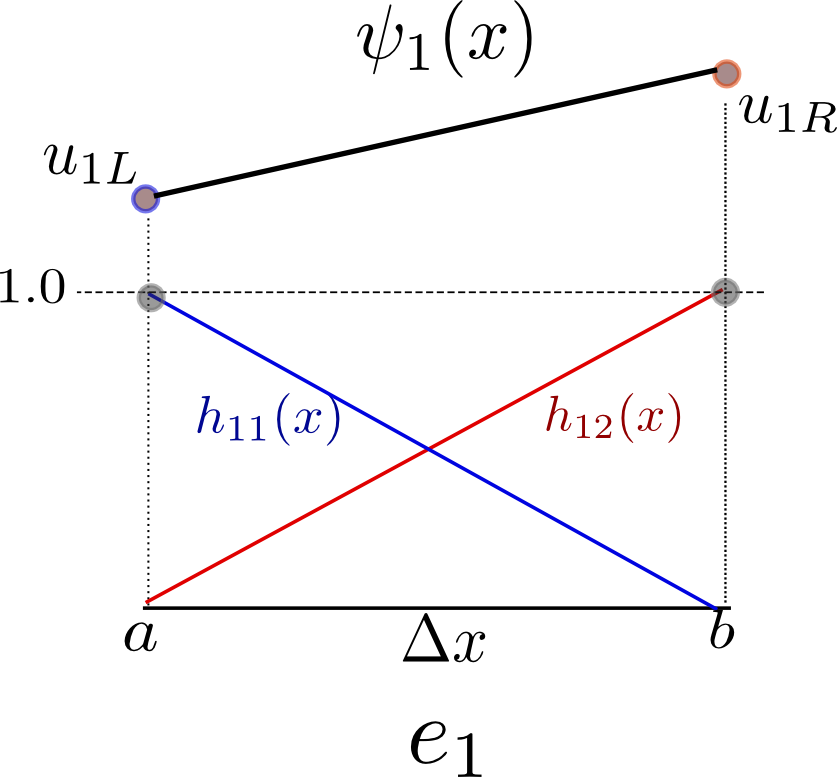
\includegraphics[width=5cm]{images/single_ele.png}
\caption{Single finite element.}
\label{single_ele}
\end{figure}

\begin{figure}[!htbp]
\centering
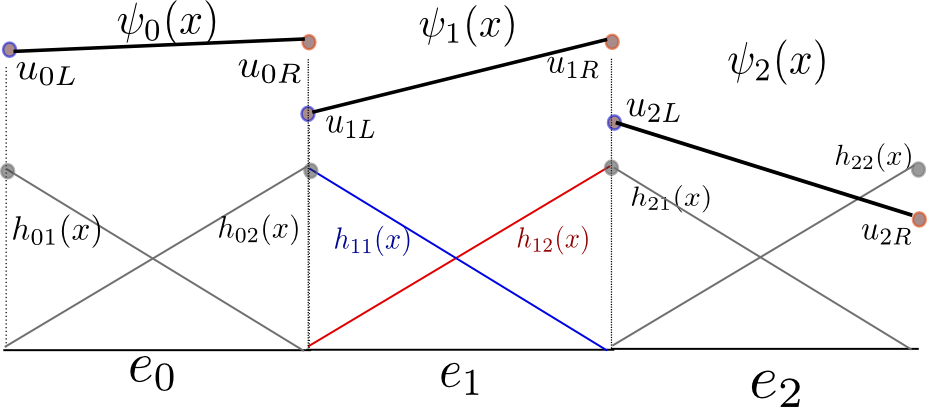
\includegraphics[width=8cm]{images/multi_ele.png}
\caption{Multiple DG finite elements.}
\label{multi_ele}
\end{figure}

In practice the transport equation is integrated element-by-element, rather than over the whole domain.  The contribution of each element will be summed together to recover the neutron balance over the whole domain.  For now, we consider an interior element, $e_1$ defined on the sub-region: $[a, b]$.  Figure \ref{multi_ele} shows the interior element $e_1$ bounded by two other elements.  Note that the hypothetical DGFE numerical solution $\psi$ jumps in value at element boundaries.  As a consequence, at element boundaries the solution is double value (in 1D, in higher dimensions it could be $N$-valued).  This is where the Discontinuous Galerkin finite element scheme differs from the more commonly known Continuous Galerkin (CG) FE spatial discretization method.